\ifnum\outputmode=0
  \def\pgfsysdriver{pgfsys-dvisvgm.def}
\fi
\documentclass[tikz,border=5pt]{standalone}

\usepackage{tikz-feynman}

\definecolor{qftink}{HTML}{26363F}
\definecolor{qftmuted}{HTML}{657B85}
\definecolor{qftsakura}{HTML}{D86483}

\tikzfeynmanset{compat=1.1.0}
\tikzset{
  qft scalar/.style={draw=qftink, line width=0.8pt},
  qft vertex/.style={circle, fill=qftsakura, draw=qftsakura,
    inner sep=1.35pt},
  topology label/.style={font=\sffamily\footnotesize, text=qftmuted},
  point label/.style={font=\small, text=qftink},
}

\begin{document}
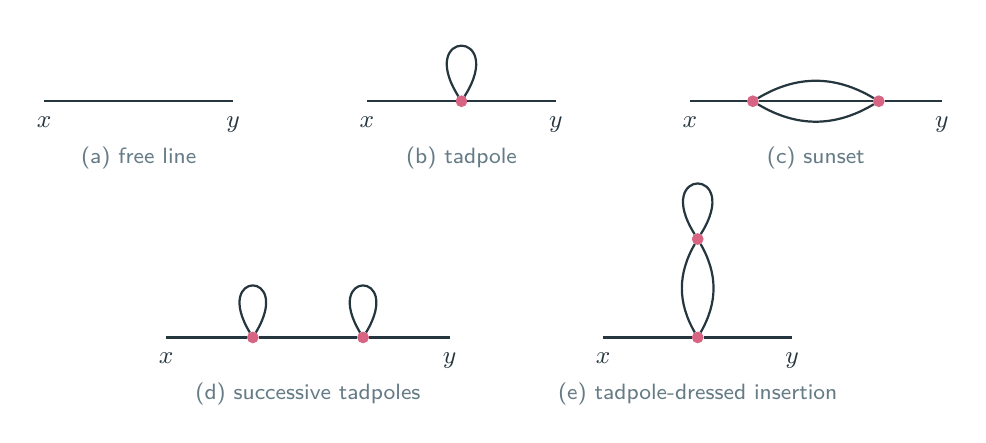
\begin{tikzpicture}[x=1cm, y=1cm]
  \begin{scope}[shift={(0,0)}]
    \begin{feynman}
      \vertex (x) at (0,0);
      \vertex (y) at (2.4,0);
      \diagram*{(x) -- [qft scalar] (y)};
    \end{feynman}
    \node[point label, below=2pt] at (x) {$x$};
    \node[point label, below=2pt] at (y) {$y$};
    \node[topology label] at (1.2,-0.72) {(a) free line};
  \end{scope}

  \begin{scope}[shift={(4.1,0)}]
    \begin{feynman}
      \vertex (x) at (0,0);
      \vertex[qft vertex] (z) at (1.2,0) {};
      \vertex (y) at (2.4,0);
      \diagram*{
        (x) -- [qft scalar] (z) -- [qft scalar] (y)
      };
    \end{feynman}
    \draw[qft scalar] (z) .. controls +(0.58,0.92) and +(-0.58,0.92) .. (z);
    \node[point label, below=2pt] at (x) {$x$};
    \node[point label, below=2pt] at (y) {$y$};
    \node[topology label] at (1.2,-0.72) {(b) tadpole};
  \end{scope}

  \begin{scope}[shift={(8.2,0)}]
    \begin{feynman}
      \vertex (x) at (0,0);
      \vertex[qft vertex] (z1) at (0.8,0) {};
      \vertex[qft vertex] (z2) at (2.4,0) {};
      \vertex (y) at (3.2,0);
      \diagram*{
        (x) -- [qft scalar] (z1),
        (z1) -- [qft scalar, bend left=31] (z2),
        (z1) -- [qft scalar] (z2),
        (z1) -- [qft scalar, bend right=31] (z2),
        (z2) -- [qft scalar] (y)
      };
    \end{feynman}
    \node[point label, below=2pt] at (x) {$x$};
    \node[point label, below=2pt] at (y) {$y$};
    \node[topology label] at (1.6,-0.72) {(c) sunset};
  \end{scope}

  \begin{scope}[shift={(1.55,-3.0)}]
    \begin{feynman}
      \vertex (x) at (0,0);
      \vertex[qft vertex] (z1) at (1.1,0) {};
      \vertex[qft vertex] (z2) at (2.5,0) {};
      \vertex (y) at (3.6,0);
      \diagram*{
        (x) -- [qft scalar] (z1) -- [qft scalar] (z2)
          -- [qft scalar] (y)
      };
    \end{feynman}
    \draw[qft scalar] (z1) .. controls +(0.52,0.86) and +(-0.52,0.86) .. (z1);
    \draw[qft scalar] (z2) .. controls +(0.52,0.86) and +(-0.52,0.86) .. (z2);
    \node[point label, below=2pt] at (x) {$x$};
    \node[point label, below=2pt] at (y) {$y$};
    \node[topology label] at (1.8,-0.72) {(d) successive tadpoles};
  \end{scope}

  \begin{scope}[shift={(7.1,-3.0)}]
    \begin{feynman}
      \vertex (x) at (0,0);
      \vertex[qft vertex] (z1) at (1.2,0) {};
      \vertex (y) at (2.4,0);
      \vertex[qft vertex] (z2) at (1.2,1.25) {};
      \diagram*{
        (x) -- [qft scalar] (z1) -- [qft scalar] (y),
        (z1) -- [qft scalar, bend left=30] (z2),
        (z1) -- [qft scalar, bend right=30] (z2)
      };
    \end{feynman}
    \draw[qft scalar] (z2) .. controls +(0.58,0.92) and +(-0.58,0.92) .. (z2);
    \node[point label, below=2pt] at (x) {$x$};
    \node[point label, below=2pt] at (y) {$y$};
    \node[topology label] at (1.2,-0.72) {(e) tadpole-dressed insertion};
  \end{scope}
\end{tikzpicture}
\end{document}
